% =============================================================================
%  Dinamica3_Fase2_Diapositiva2.tex — Dinámica 3, Fase 2, Diapositiva 2:
%  el filtro del hiperfoco. Las líneas de la novela tradicional se difuminan
%  en gris; los pensamientos de Oliveira quedan nítidos y resaltados.
%  Fuente: Cortázar, Rayuela, Alfaguara, p. 212, líneas 1–16.
%  Formato 16:9. Compilar con: bash ../../../compilar_diapositivas.sh
% =============================================================================
\documentclass[tikz,border=0pt]{standalone}
\usepackage[utf8]{inputenc}
\usepackage[T1]{fontenc}
\usepackage{ebgaramond}
\usetikzlibrary{fadings}

% ── Parámetros ────────────────────────────────────────────────────────────────
%  \Difuminado: intensidad del desenfoque de la novela (0 = nítido, 1 = ilegible)
\def\Difuminado{0.35}
\def\RadioMax{5}        % radio máximo del desenfoque, en pt (con \Difuminado = 1)
\def\TamLetra{20}       % tamaño de letra, en pt
\def\Interlinea{27.5}   % interlineado, en pt

% ── Paleta ────────────────────────────────────────────────────────────────────
\definecolor{Pergamino}{HTML}{F1EBDD}
\definecolor{PergaminoBorde}{HTML}{DCCFB4}
\definecolor{Fibra}{HTML}{B9A27A}
\definecolor{Tinta}{HTML}{2B2620}
\definecolor{Novela}{HTML}{7D766C}      % gris cálido para la novela
\definecolor{Resalte}{HTML}{FFE14D}
\definecolor{Referencia}{HTML}{6B5A43}
\definecolor{BokehDorado}{HTML}{E8B04B}
\definecolor{BokehAmbar}{HTML}{D9893A}
\definecolor{BokehCrema}{HTML}{FFF8E7}

% ── Dimensiones (16:9) ────────────────────────────────────────────────────────
\def\ancho{32}
\def\alto{18}

% ── Marcado del texto ─────────────────────────────────────────────────────────
%  \Nov{...}: línea de la novela (capa difusa).  \Oli{...}: línea de Oliveira
%  (capa nítida, con resalte). Ambas reservan el mismo margen \fboxsep para que
%  las dos capas coincidan en posición.
\newif\ifcapanitida
\newcommand{\Nov}[1]{\hspace*{\fboxsep}\ifcapanitida\phantom{#1}\else#1\fi}
\newcommand{\Oli}[1]{%
  \ifcapanitida\colorbox{Resalte!55}{\textcolor{Tinta}{#1}}%
  \else\phantom{\colorbox{Resalte}{#1}}\fi}

\newcommand{\Bloque}{%
  \Nov{En setiembre del 80, pocos meses después del fallecimiento}\\
  \Oli{Y las cosas que lee, una novela, mal escrita, para colmo una edi-}\\
  \Nov{de mi padre, resolví apartarme de los negocios, cediéndolos a}\\
  \Oli{ción infecta, uno se pregunta cómo puede interesarle algo así.}\\
  \Nov{otra casa extractora de Jerez tan acreditada como la mía; realicé}\\
  \Oli{Pensar que se ha pasado horas enteras devorando esta sopa fría y}\\
  \Nov{los créditos que pude, arrendé los predios, traspasé las bodegas}\\
  \Oli{desabrida, tantas otras lecturas increíbles, \textit{Elle} y \textit{France Soir}, los}\\
  \Nov{y sus existencias, y me fui a vivir a Madrid. Mi tío (primo car-}\\
  \Oli{tristes magazines que le prestaba Babs. Y \textit{me fui a vivir a Madrid},}\\
  \Nov{nal de mi padre), don Rafael Bueno de Guzmán y Ataide, quiso}\\
  \Oli{me imagino que después de tragarse cinco o seis páginas uno}\\
  \Nov{albergarme en su casa; mas yo me resistí a ello por no perder mi}\\
  \Oli{acaba por engranar y ya no puede dejar de leer, un poco como}\\
  \Nov{independencia. Por fin supe hallar un término de conciliación,}\\
  \Oli{no se puede dejar de dormir o de mear, servidumbres o látigos o […]}%
}

\begin{document}
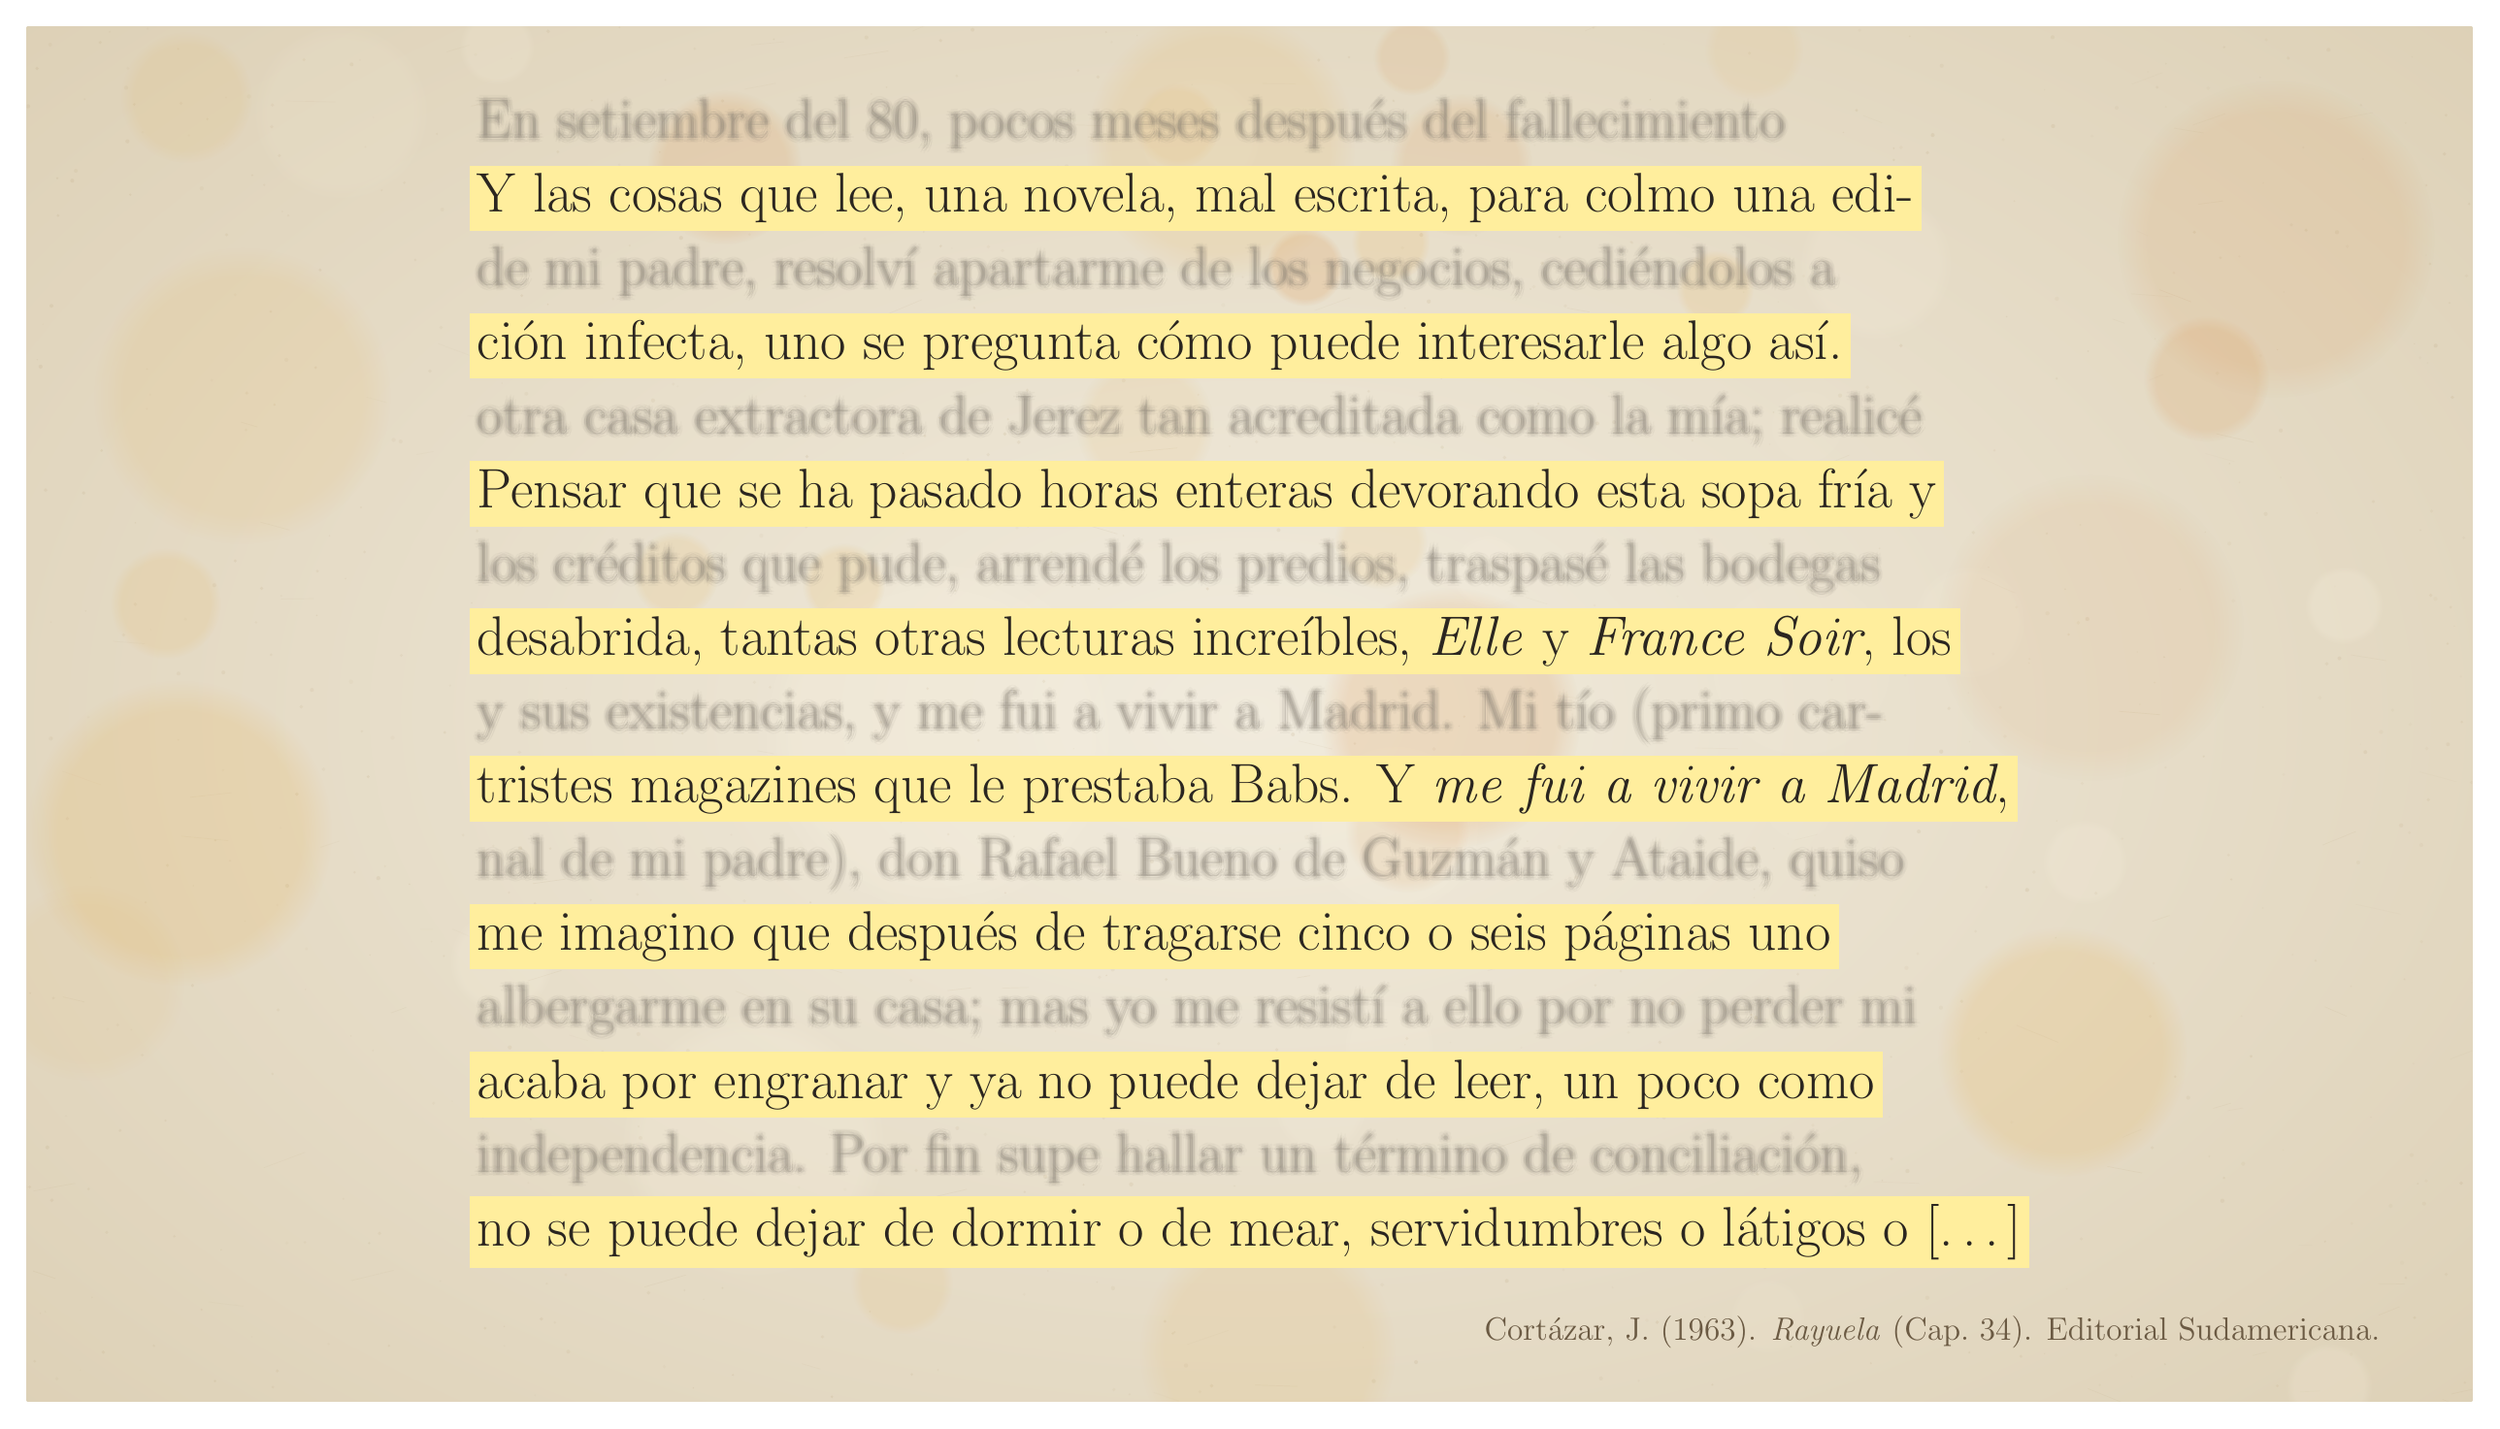
\begin{tikzpicture}
  \useasboundingbox (0,0) rectangle (\ancho,\alto);
  \clip (0,0) rectangle (\ancho,\alto);

  % Fondo con viñeta
  \fill[PergaminoBorde] (0,0) rectangle (\ancho,\alto);
  \shade[inner color=Pergamino, outer color=PergaminoBorde]
    (\ancho/2,\alto/2) ellipse [x radius=0.72*\ancho, y radius=0.80*\alto];

  % Textura (misma semilla que la Fase 1)
  \pgfmathsetseed{1914}
  \foreach \i in {1,...,900}{
    \pgfmathsetmacro{\x}{rnd*\ancho}
    \pgfmathsetmacro{\y}{rnd*\alto}
    \pgfmathsetmacro{\r}{0.008+0.02*rnd}
    \pgfmathsetmacro{\o}{0.05+0.12*rnd}
    \fill[Fibra, opacity=\o] (\x,\y) circle (\r);
  }
  \foreach \i in {1,...,140}{
    \pgfmathsetmacro{\x}{rnd*\ancho}
    \pgfmathsetmacro{\y}{rnd*\alto}
    \pgfmathsetmacro{\l}{0.15+0.5*rnd}
    \pgfmathsetmacro{\a}{-25+50*rnd}
    \pgfmathsetmacro{\o}{0.04+0.08*rnd}
    \draw[Fibra, opacity=\o, line width=0.25pt, rotate around={\a:(\x,\y)}]
      (\x,\y) -- ++(\l,0);
  }

  % Bokeh cálido y sutil (misma semilla que la Fase 1, Diapositiva 2)
  \pgfmathsetseed{2026}
  \foreach \i in {1,...,45}{
    \pgfmathsetmacro{\x}{rnd*\ancho}
    \pgfmathsetmacro{\y}{rnd*\alto}
    \pgfmathsetmacro{\r}{0.5+1.9*rnd^2}
    \pgfmathsetmacro{\o}{0.06+0.12*rnd}
    \pgfmathtruncatemacro{\c}{int(3*rnd)}
    \ifcase\c\relax \def\col{BokehDorado}\or \def\col{BokehAmbar}%
      \else \def\col{BokehCrema}\fi
    \fill[\col, fill opacity=\o, path fading=circle with fuzzy edge 20 percent]
      (\x,\y) circle (\r);
  }

  % Estilo común del bloque
  \tikzset{bloque/.style={anchor=center, align=left, inner sep=0pt,
    font=\fontsize{\TamLetra}{\Interlinea}\selectfont}}
  \coordinate (centro) at (\ancho/2,\alto/2+0.4);

  % Capa difusa: la novela, en gris y con desenfoque simulado
  \pgfmathsetmacro{\R}{\Difuminado*\RadioMax}
  \capanitidafalse
  \foreach \ang in {0,45,...,315}{
    \foreach \f/\op in {1/0.05, 0.5/0.07}{
      \node[bloque, text=Novela, text opacity=\op]
        at ([shift={(\ang:\f*\R pt)}]centro) {\Bloque};
    }
  }
  \node[bloque, text=Novela, text opacity={0.35*(1-\Difuminado)}]
    at (centro) {\Bloque};

  % Capa nítida: los pensamientos de Oliveira
  \capanitidatrue
  \node[bloque] at (centro) {\Bloque};

  % Referencia APA
  \node[anchor=south east, text=Referencia, inner sep=0pt,
        font=\fontsize{13}{16}\selectfont]
    at (\ancho-1.2,0.7)
    {Cortázar, J. (1963). \textit{Rayuela} (Cap.~34). Editorial Sudamericana.};
\end{tikzpicture}
\end{document}
